\begin{figure}[H]
    \centering
    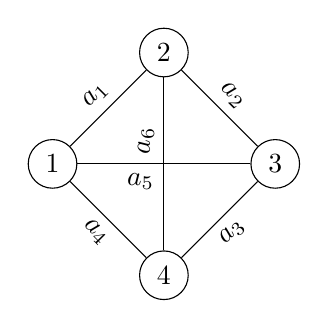
\begin{tikzpicture}[node distance={20mm}, main/.style = {draw, circle}]
    \node[main] (1) {$1$}; 
    \node[main] (2)[above right of=1] {$2$};
    \node[main] (3)[below right of=2] {$3$};
    \node[main] (4)[below left of=3] {$4$};
    \draw (1) -- node [midway, above, sloped] {$a_1$}(2);
    \draw (2) -- node [ above, midway, sloped] {$a_2$}(3);
    \draw (3) -- node [ below, midway, sloped] {$a_3$}(4);
    \draw (4) -- node [ below, midway, sloped] {$a_4$}(1);
    \draw (4) -- node [ above right, midway, sloped] {$a_6$}(2);
    \draw (1) -- node [ below left, midway, sloped] {$a_5$}(3);
    \end{tikzpicture}\\
    \caption{$K_4$}
    \label{ex4:image}
\end{figure}